\documentclass[border=6pt]{standalone}
\usepackage{tikz}
\usetikzlibrary{arrows.meta}
\begin{document}
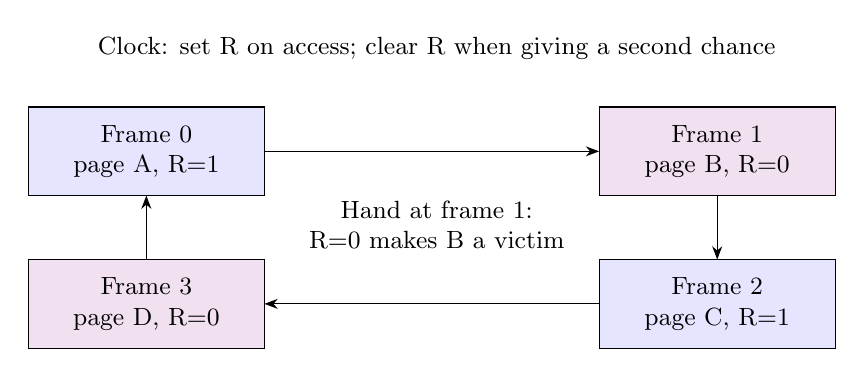
\begin{tikzpicture}[>=Stealth]
\node[align=center,font=\small] at (6.438,4.625) {Clock: set R on access; clear R when giving a second chance};
\draw[fill=blue!10] (1.250,3.875) rectangle (4.250,2.750);
\node[align=center,font=\small] at (2.750,3.312) {Frame 0\\page A, R=1};
\draw[fill=violet!12] (8.500,3.875) rectangle (11.500,2.750);
\node[align=center,font=\small] at (10.000,3.312) {Frame 1\\page B, R=0};
\draw[fill=blue!10] (8.500,1.938) rectangle (11.500,0.812);
\node[align=center,font=\small] at (10.000,1.375) {Frame 2\\page C, R=1};
\draw[fill=violet!12] (1.250,1.938) rectangle (4.250,0.812);
\node[align=center,font=\small] at (2.750,1.375) {Frame 3\\page D, R=0};
\draw[->] (4.250,3.312) -- (8.500,3.312);
\draw[->] (10.000,2.750) -- (10.000,1.938);
\draw[->] (8.500,1.375) -- (4.250,1.375);
\draw[->] (2.750,1.938) -- (2.750,2.750);
\node[align=center,font=\small] at (6.438,2.375) {Hand at frame 1:\\R=0 makes B a victim};
\end{tikzpicture}
\end{document}
